%\documentclass[a4j,10pt]{ujarticle}
\RequirePackage{ifuptex,ifluatex}
\ifluatex
\documentclass{ltjsarticle}
\else
\ifupTeX
\documentclass[uplatex,dvipdfmx]{jsarticle}
\else
\documentclass[dvipdfmx]{jsarticle}
\fi
\fi
%\usepackage[dviout]{graphicx}
\usepackage{graphicx}
%%%%%%%%%%%%%%%%%%%%%%%%%%%%%%%%%%%%%%%%%%%%%%%%%%%%%%%%%%%%%%%%%%%%%

\pagestyle{empty}
\sloppy\fussy
\setlength{\topmargin}{-20.4mm}
\setlength{\textheight}{271mm}
\setlength{\textwidth}{175mm}
\setlength{\oddsidemargin}{-5.4mm}
\setlength{\evensidemargin}{-5.4mm}
\setlength{\headheight}{0mm}
\setlength{\footskip}{10mm}
\renewcommand{\baselinestretch}{1.0}
\renewcommand{\textfraction}{0}\renewcommand{\floatpagefraction}{1}
\renewcommand{\topfraction}{1} \renewcommand{\bottomfraction}{1}
%%%%%%%%%%%%%%%%%%%%%%%%%%%%%%%%%%%%%%%%%%%%%%%%%%%%%%%%%%%%%%%%%%%%%
\begin{document} 
\twocolumn[
\begin{center}
{\Large TCP並列接続を用いたプログレッシブダウンロード\\における順序制御方式の実装}\\
\vspace{0.1cm}
{\large Implementation of sequence control method in progressive download \\
	using parallel TCP connection}\\
\vspace{0.2cm}
{\large 1420180  平城 光雄 Mitsuo Heijo}\\
{\large 指導教員\ \  舟阪 淳一}\\
\end{center}
]
\section{はじめに}
近年,Webコンテンツの大容量化が顕著である.
効率的なコンテンツの配信方法としてCDNを利用したコンテンツ分散配置などがすでに運用されている.
このように同一のコンテンツが様々な場所に配置されていることを利用して複数のWebサーバーと同時並行的に通信を行うことで,より高速で通信を実現しようとする方法が提案されている.
本研究では,性能の異なる複数のTCP接続を利用して同一のファイルを分割取得する場合を想定し,リクエスト送信時に,各TCP接続間の性能を比較し到着順序逆転の発生を抑制する能動的な順序制御方式を提案し,HTTPクライアントとして実装し評価する.

\section{提案手法}
確立したTCP接続群の中で性能の最も高いTCP接続には,最も若番のブロックを要求する.
性能の低いTCP接続では前回のブロック要求の送信からブロックの到着までの間隔を算出し,
その算出値に基づいて後ろのブロックを遅延要求する.
図\ref{delay}にその模式図を示す.

\begin{figure}[ht]
	\centering
	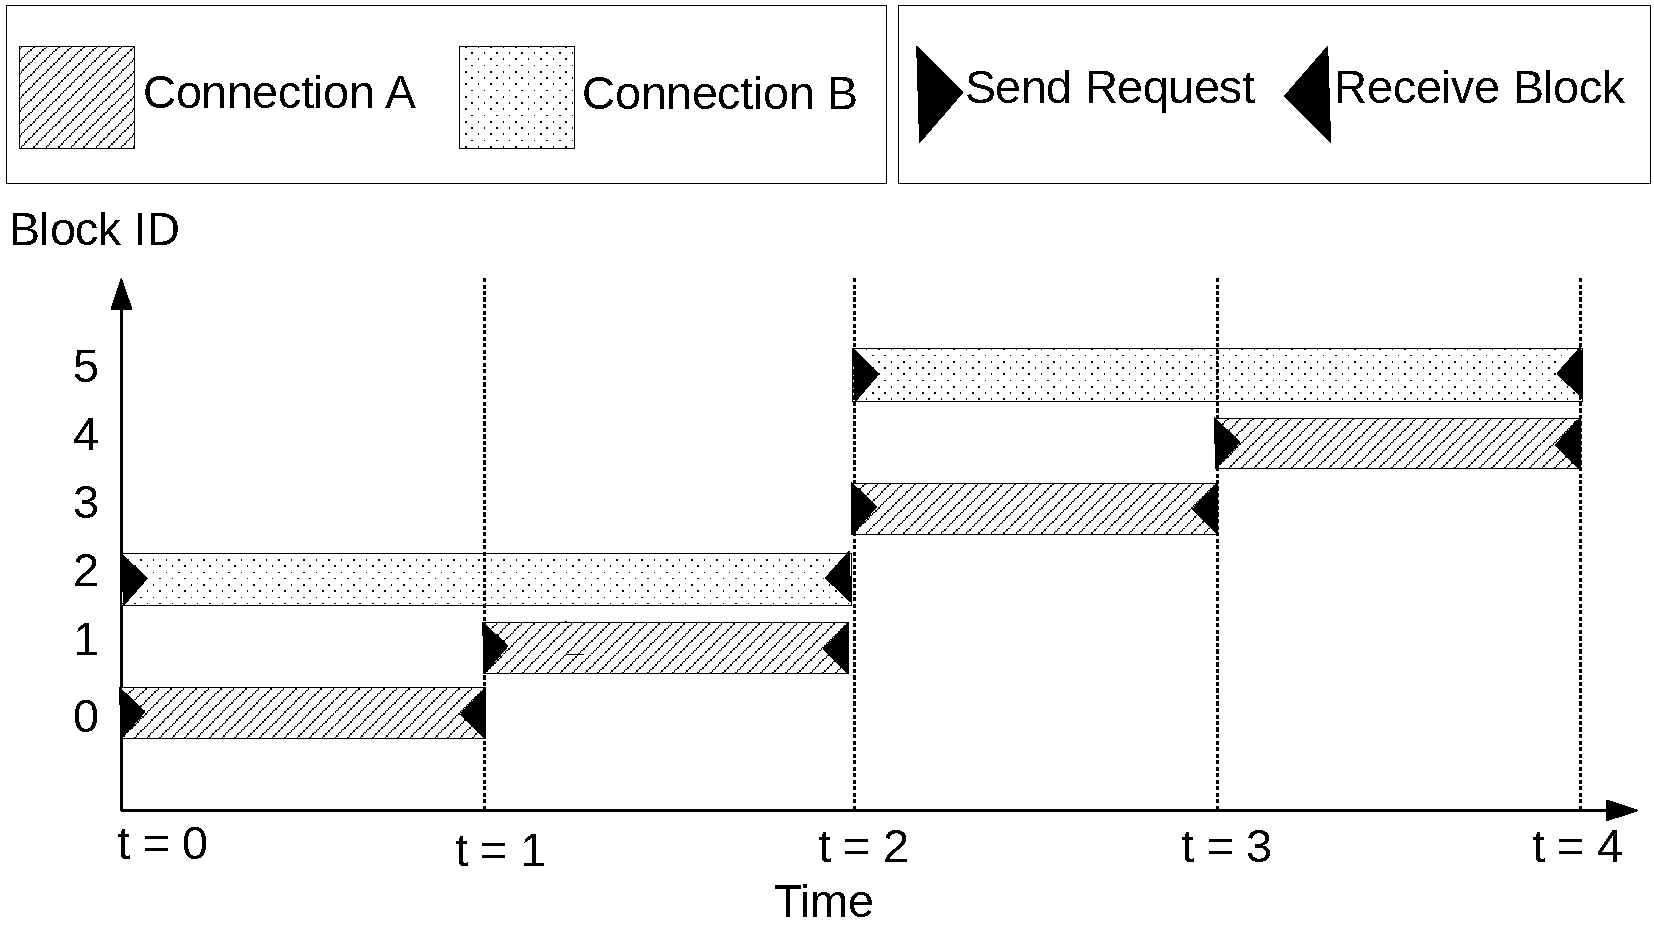
\includegraphics[width=8cm]{figure/delay.pdf}
	\caption{遅延要求の模式図}
	\label{delay}
\end{figure}

\section{評価}
パブリックネットワークでの評価にあたり,Ubuntuのリリースイメージファイルの配布に用いられているパブリックミラー\cite{ubuntu}を利用した.
複数のミラーから同一のイメージファイルを分割して取得する際の順序逆転の影響を評価する.

\begin{table}[htbp]
	\begin{center}
		\caption{使用したパブリックミラー一覧}
		\label{tablemirror}
		\scalebox{0.7}[0.7]{
		\begin{tabular}{|l|l|l|} \hline
			ホスト & 組織 & 国\\ \hline \hline
			ftp.jaist.ac.jp & JAIST & JP \\
			ubuntutym2.u-toyama.ac.jp & Univercity of Toyama & JP \\
			releases.ubuntu.com & Canonical & GB \\
			mirrorservice.org & University of Kent & GB \\
			ubuntu.ipacct.com & IPACCT & BG \\
			mirror.pop-sc.rnp.br & PoP-SC & BR \\
			ftp.belnet.be & Belnet & BE \\
			mirrors.mit.edu & MIT & US \\
			mirror.yandex.ru & Yandex & RU \\ \hline
		\end{tabular}}
	\end{center}
\end{table}

\begin{figure}[ht]
	\centering
	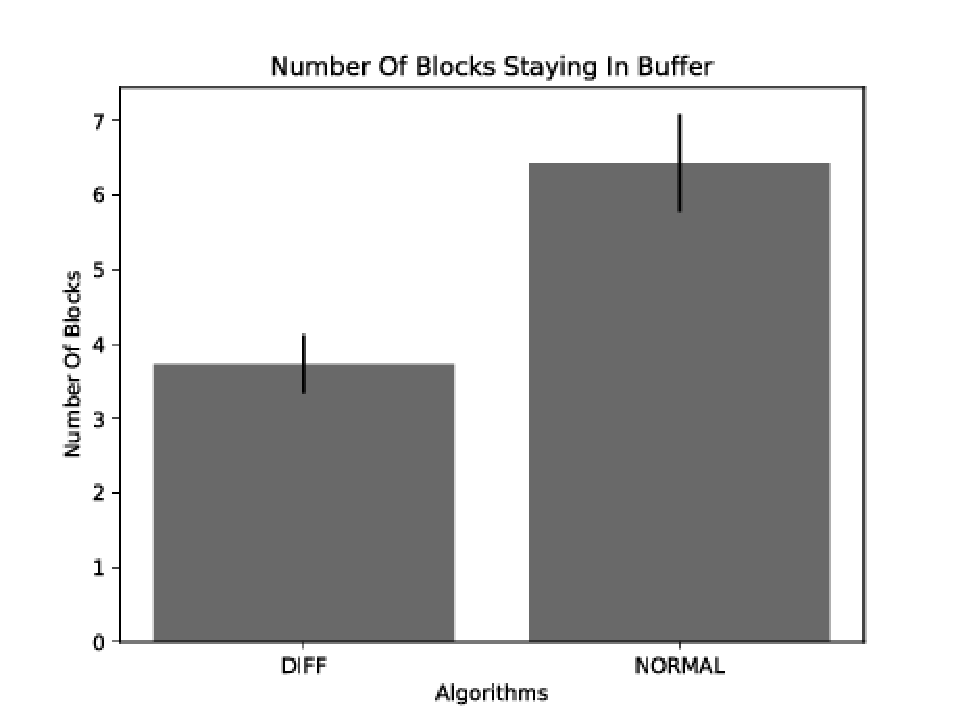
\includegraphics[width=7cm]{figure/nsb-g.pdf}
	\caption{平均非有効ブロック数}
	\label{nsbpub}
\end{figure}

\section{まとめ}
パブリックネットワークでの評価では差分計測を用いた遅延予測方式は初期遅延予測方式と組み合わせることで制御なしの場合と比べて,50\%の初期バッファリング時間の削減,30\%の非有効ブロック数の削減と50\%の平均遅延時間の削減が確認できた.

%%%%%%%%%%%%%%%%%%%%%%%%%%%%%%%%%%%%%%%%%%%%%%%%%%%%%%%%%%%%%%%%%%%%%%%%%%
% 参考文献
%%%%%%%%%%%%%%%%%%%%%%%%%%%%%%%%%%%%%%%%%%%%%%%%%%%%%%%%%%%%%%%%%%%%%%%%%%
\begin{thebibliography}{2}
\bibitem{proxy}
Junichi Funasaka, Atsushi Kawano, and Kenji Ishida: Adaptive Parallel Downloading Method for Proxy Systems, IEICE Trans., Vol.E90-B, No.4, pp.720-727, Apr. 2007.
\bibitem{ubuntu}
Official CD Mirrors for Ubuntu available at., https://launchpad.net/ubuntu/+cdmirrors, 2018.
\end{thebibliography}

\end{document}
